% Template file for an a0 landscape poster.
% Written by Graeme, 2001-03 based on Norman's original microlensing
% poster.
%
% See discussion and documentation at
% <http://www.astro.gla.ac.uk/users/norman/docs/posters/> 
%
% $Id: poster-template-landscape.tex,v 1.2 2002/12/03 11:25:46 norman Exp $


% Default mode is landscape, which is what we want, however dvips and
% a0poster do not quite do the right thing, so we end up with text in
% landscape style (wide and short) down a portrait page (narrow and
% long). Printing this onto the a0 printer chops the right hand edge.
% However, 'psnup' can save the day, reorienting the text so that the
% poster prints lengthways down an a0 portrait bounding box.
%
% 'psnup -w85cm -h119cm -f poster_from_dvips.ps poster_in_landscape.ps'

\documentclass[a0]{a0poster}
% You might find the 'draft' option to a0 poster useful if you have
% lots of graphics, because they can take some time to process and
% display. (\documentclass[a0,draft]{a0poster})
\input defs
\pagestyle{empty}
\setcounter{secnumdepth}{0}
\renewcommand{\familydefault}{\sfdefault}
\newcommand{\QED}{~~\rule[-1pt]{8pt}{8pt}}\def\qed{\QED}

\renewcommand{\reals}{{\mbox{\bf R}}}

% The textpos package is necessary to position textblocks at arbitary 
% places on the page.
\usepackage[absolute]{textpos}

\usepackage{fleqn,psfrag,wrapfig,tikz}
\usepackage{amsmath, xparse}

\usepackage[pdftex,unicode, 
colorlinks=true,
linkcolor = blue]{hyperref}

\usepackage{animate}
\usepackage{wrapfig} 
\usepackage{caption}

\usepackage{algorithm}
\usepackage{algpseudocode}
\usepackage{nicefrac} 


\usepackage[papersize={38in,28in}]{geometry}

% Graphics to include graphics. Times is nice on posters, but you
% might want to switch it off and go for CMR fonts.
\usepackage{graphics}


% we are running pdflatex, so convert .eps files to .pdf
%\usepackage[pdftex]{graphicx}
%\usepackage{epstopdf}

% These colours are tried and tested for titles and headers. Don't
% over use color!

\usepackage{color}
\definecolor{Red}{rgb}{0.9,0.0,0.1}

\definecolor{bluegray}{rgb}{0.15,0.20,0.40}
\definecolor{bluegraylight}{rgb}{0.35,0.40,0.60}
\definecolor{gray}{rgb}{0.3,0.3,0.3}
\definecolor{lightgray}{rgb}{0.7,0.7,0.7}
\definecolor{darkblue}{rgb}{0.2,0.2,1.0}
\definecolor{darkgreen}{rgb}{0.0,0.5,0.3}

\renewcommand{\labelitemi}{\textcolor{bluegray}\textbullet}
\renewcommand{\labelitemii}{\textcolor{bluegray}{--}}

\setlength{\labelsep}{0.5em}


% see documentation for a0poster class for the size options here
\let\Textsize\normalsize
%\def\Head#1{\noindent\hbox to \hsize{\hfil{\LARGE\color{bluegray} #1}}\bigskip}
\def\Head#1{\noindent{\LARGE\color{bluegray} #1}\bigskip}
\def\LHead#1{\noindent{\LARGE\color{bluegray} #1}\bigskip}
\def\Subhead#1{\noindent{\large\color{bluegray} #1}\bigskip}
\def\Title#1{\noindent{\VeryHuge\color{Red} #1}}

\floatname{algorithm}{Algorithm}
\renewcommand{\algorithmicrequire}{\textbf{Input:}}
\renewcommand{\algorithmicensure}{\textbf{return}}
\renewcommand{\algorithmicfunction}{\textbf{def}}
\algtext*{EndFunction}

\newcommand{\etal}{\textit{et al}.}
\newcommand{\TODO}[1]{{\color{red}TODO: #1}}
\newcommand{\NOTE}[1]{{\color{blue}NOTE: #1}}
\newtheorem{theorem}{Theorem}
%\newtheorem*{theorem*}{Theorem}
\newcommand{\tr}{\textnormal{tr}}
\newcommand\E{\mathbb{E}}
\newcommand\R{\mathbb{R}}

\renewcommand{\epsilon}{\varepsilon}

\newcommand*{\matr}[1]{\mathbfit{#1}}
\newcommand*{\tran}{^{\mkern-1.5mu\mathsf{T}}}
\newcommand*{\conj}[1]{\overline{#1}}
\newcommand*{\hermconj}{^{\mathsf{H}}}

\newcommand{\vx}{\mathbf{x}}
\newcommand{\vepsilon}{\mathbf{\epsilon}}
\newcommand{\vtheta}{\mathbf{\theta}}%
\newcommand{\vpsi}{{\bm{\psi}}}
\newcommand{\vpi}{{\bm{\pi}}}
\newcommand{\vphi}{{\bm{\phi}}}
\newcommand\bigO{\mathcal{O}}
\newcommand{\va}{\mathbf{a}}
\newcommand{\vh}{\mathbf{h}}
\newcommand{\vz}{\mathbf{z}}
\newcommand{\vX}{\mathbf{X}}
\newcommand{\vw}{\mathbf{w}}
\newcommand{\vv}{\mathbf{v}}
\newcommand{\vr}{\mathbf{r}}
\newcommand{\vg}{\mathbf{g}}
\newcommand{\vI}{\mathbf{I}}
\newcommand{\vzero}{\bf{0}}
%\newcommand{\ones}[1]{\mat{1}_{#1}}
\newcommand{\eye}[1]{\mat{E}_{#1}}
\newcommand{\tra}{^{\mathsf{T}}}
\newcommand{\vect}[1]{{\bf{#1}}}
\newcommand{\mat}[1]{\mathbf{#1}}
\newcommand{\pderiv}[2]{\frac{\partial #1}{\partial #2}}
\newcommand{\npderiv}[2]{\nicefrac{\partial #1}{\partial #2}}
%\newcommand{\argmin}{\operatornamewithlimits{argmin}}
%\newcommand{\argmax}{\operatornamewithlimits{argmax}}
\newcommand{\expect}{\mathbb{E}}
\newcommand{\expectargs}[2]{\mathbb{E}_{#1} \left[ {#2} \right]}
\newcommand{\var}{\mathbb{V}}
\newcommand{\varL}{\mathcal{L}}
\def\iid{i.i.d.\ }
\def\simiid{\overset{\mbox{\tiny iid}}{\sim}}
\newcommand{\defeq}{\mathrel{:\mkern-0.25mu=}}
\newcommand{\Normal}{\mathcal{N}}
\newcommand{\Nt}[3]{\mathcal{N}\!\left(#1 \middle| #2,#3\right)}
\newcommand{\N}[2]{\mathcal{N}\!\left(#1,#2\right)}
\DeclareMathOperator{\KLop}{KL}
\newcommand{\KL}[2]{\KLop \left(#1 \middle \| #2 \right)}
\newcommand{\tunderbrace}[1]{\underbrace{\textstyle #1}}


\newcommand{\latent}{\vz}
\newcommand{\hidden}{\vh}
\newcommand{\obs}{\vx}
\newcommand{\sol}{\vz}  %
\newcommand{\obsdim}{D_x}
\newcommand{\latentdim}{D}
\newcommand{\solvefunc}{\textnormal{ODESolve}}
\newcommand{\tstart}{{t_\textnormal{0}}}
\newcommand{\tend}{{t_\textnormal{1}}}
\newcommand{\lograte}{\lambda}%
\newcommand{\method}{Latent ODE}
\newcommand{\cnfx}{\sol}
\newcommand{\adj}{\va}


% Set up the grid
%
% Note that [40mm,40mm] is the margin round the edge of the page --
% it is _not_ the grid size. That is always defined as 
% PAGE_WIDTH/HGRID and PAGE_HEIGHT/VGRID. In this case we use
% 23 x 12. This gives us three columns of width 7 boxes, with a gap of
% width 1 in between them. 12 vertical boxes is a good number to work
% with.
%
% Note however that texblocks can be positioned fractionally as well,
% so really any convenient grid size can be used.
%
\TPGrid[40mm,40mm]{23}{12}      % 3 cols of width 7, plus 2 gaps width 1

\parindent=0pt
\parskip=0.2\baselineskip

\begin{document}

% Understanding textblocks is the key to being able to do a poster in
% LaTeX. In
%
%    \begin{textblock}{wid}(x,y)
%    ...
%    \end{textblock}
%
% the first argument gives the block width in units of the grid
% cells specified above in \TPGrid; the second gives the (x,y)
% position on the grid, with the y axis pointing down.

% You will have to do a lot of previewing to get everything in the 
% right place.

% This gives good title positioning for a portrait poster.
% Watch out for hyphenation in titles - LaTeX will do it
% but it looks awful.
\begin{textblock}{23}(0,0)
\Title{NeuralODE studying}
\end{textblock}

\begin{textblock}{23}(0,0.6)
{
\LARGE
Ilya Lopatin
}

{
\Large
\color{bluegray}
\emph{Optimization Class Project. MIPT}
}
\end{textblock}


% Uni logo in the top right corner. A&A in the bottom left. Gives a
% good visual balance, but you may want to change this depending upon
% the graphics that are in your poster.
%\begin{textblock}{2}(0,10)
%Your logo here
%%\includegraphics{/usr/local/share/images/AandA.epsf}
%\end{textblock}

%\begin{textblock}{2}(21.2,0)
%Another logo here
%%\resizebox{2\TPHorizModule}{!}{\includegraphics{/usr/local/share/images/GUVIu/GUVIu.eps}}
%\end{textblock}


\begin{textblock}{7.0}(0,1.2)

\hrule\medskip
\Head{Introduction}\\
The NeuralODE architecture of was created in paper \cite{NeuralODE}, 2018. This project is devoted to studying of this neural network's architecture and carrying out numerical experiments with it.

\medskip
\hrule\medskip
\Head{The basic mathematical ideas of NeuralODE}\\
We can see that forward propagation in residual neural network looks like Euler's method of numerical solving of ordinary differential equation (1). It turns out that calculating gradient is presented as a solution of the other (\textit{adjoint}) ODE (2):
\begin{center}
\begin{minipage}[h]{0.4\linewidth}
\begin{equation}
\left\{\begin{array}{lr}
         \frac{d z(t) }{dt}  = f(z(t), t, \theta), \\
         t   \in [t_1 ; t_2], \\
         z(t_1)  = x
        \end{array} \right. 
\end{equation}
\end{minipage}
\hfill
\begin{minipage}[h]{0.4\linewidth}
\begin{equation}
\left\{ \begin{array}{lr}
  		 \frac{d a(t)}{dt} = - a^T(t) \frac{\partial f}{ z(t)} \\
		 a(t_2) = \frac{\partial L}{ \partial y}
\end{array} \right. 
\end{equation}
\end{minipage}
\end{center}

where $ f(z(t), t, \theta)$ is representation of neural network, $\theta$ is set of trainable parameters and $L = L(y(x))$ is loss function. The euation (3) gives us possibility to calculate gradient $\nabla_{\theta} L $ and do the procedures of gradient descent.
\begin{equation}
 \nabla_{\theta} L = \int_{t_1}^{t_2} a^T(t) \frac{\partial f}{\partial \theta} \left( z(t), t, \theta \right) dt .
\end{equation}
Below we can see the algorithm of the calculation gradient loss function.
\end{textblock}
\medskip
\hrule\medskip

\begin{textblock}{7.0}(0,6.4)
  \captionof{algorithm}{ \noindent Reverse-mode derivative of an ODE initial value problem:}
  \begin{algorithmic}[1]
\Require dynamics parameters $\theta$, start time $\tstart$, stop time $\tend$, final state $\sol(\tend)$, loss gradient $\nicefrac{\partial L}{\partial \sol(\tend)}$
\State $s_0 = [\sol(\tend), \frac{\partial L}{\partial \sol(\tend)}, {\vzero}_{|\theta|}]$ \Comment{Define initial augmented state}
\Function{\textnormal{aug\_dynamics}}{$[\sol(t), \adj(t), \cdot], t, \theta$}: \Comment{Define dynamics on augmented \hspace*{20cm}  state}
\State \textbf{return} $[f(\sol(t), t, \theta), -\adj(t)\tran{} \frac{\partial f}{\partial \sol}, -\adj(t)\tran{} \frac{\partial f}{\partial \theta}]$ \Comment{Compute \hspace*{16.7cm} vector-Jacobian products}
\EndFunction %
\State $[\sol(t_0), \frac{\partial L}{\partial \sol(t_0)}, \frac{\partial L}{\partial \theta}] = \solvefunc(s_0, \textnormal{aug\_dynamics}, \tend, \tstart, \theta)$ \Comment{Solve \hspace*{19.1cm} reverse-time ODE}
\Ensure $\frac{\partial L}{\partial \sol(t_0)}, \frac{\partial L}{\partial \theta}$ \Comment{Return gradients}
  \end{algorithmic}
  \medskip
\hrule\medskip
\end{textblock}

\begin{textblock}{7.0}(0,9.3)
\Head{Possible applications}
\begin{itemize}
\item Replacing  Res-block with NeuralODE block for using more powerfully solvers.
\item Restoring a hidden dynamics function by given set of observations.
\item Continuous normalizing flows, modeling or sampling of unknown probability density function by given points. The most common methods have $O(d^3)$  time asymptomatic when $d$ is dimension of space. The following statement turns out to be useful for reducing time costs to $O(d)$ (see \cite{NeuralODE}): \\
\hspace{1.25 cm} \textit{Let $z(t)$ be a finite continuous random variable with probability $p(z(t))$ dependent on time. Let $ dz / dt = f(z(t), t)$ be a differential equation describing a continuous-in-time transformation of $z(t)$. Assuming that $f$ is uniformly Lipschitz continuous in $z$ and continuous in $t$, then the change in $\log$ probability also follows a differential equation (4) }:
\begin{equation}
 \frac{\partial \log p \left( z(t) \right) }{\partial t } = -tr \left( \frac{\partial f }{ \partial z(t) }   \right)
 \end{equation} 
\end{itemize}
\end{textblock}

\begin{textblock}{7.0}(8,1.2)
\hrule\medskip
\Head{Restoring the hidden dynamics function}\\
If we have some set of given observations or points of hidden distribution density, the adjoint sensitivity method solves an augmented ODE backwards in time. \begin{wrapfigure}{r}{0.5\linewidth}
\centering
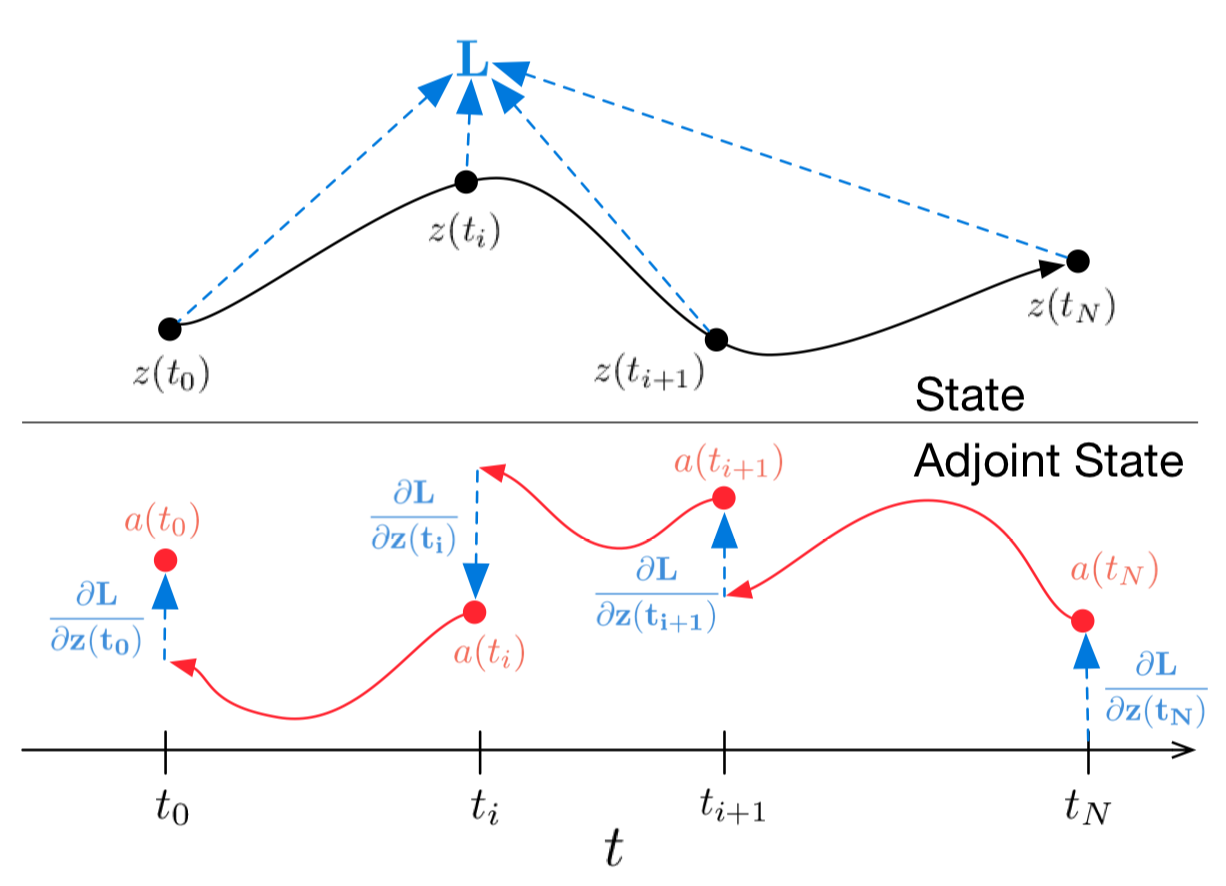
\includegraphics[width = 1\linewidth]{figures/backprop.png}
\caption{}
\end{wrapfigure} The augmented system contains both the original state and the sensitivity of the loss with respect to the state. If the loss depends directly on the state at multiple observation times, the adjoint state must be updated in the direction of the partial derivative of the loss with respect to each observation, see figure 1.

Note that during the experiments, the following problem was found. Let the hidden dynamics function conform to the equation $z' = A z$ if the constant matrix $A$ has an eigenvalue  with a positive real part, which means that the system is unstable, then the program crashes. Author's comment about it: \textit{This underflow error indicates that the system is too stiff for an explicit method to solve. The step size needs to be extremely small in order to satisfy the desired tolerance. Ricky Chen }

\begin{figure}
\centering
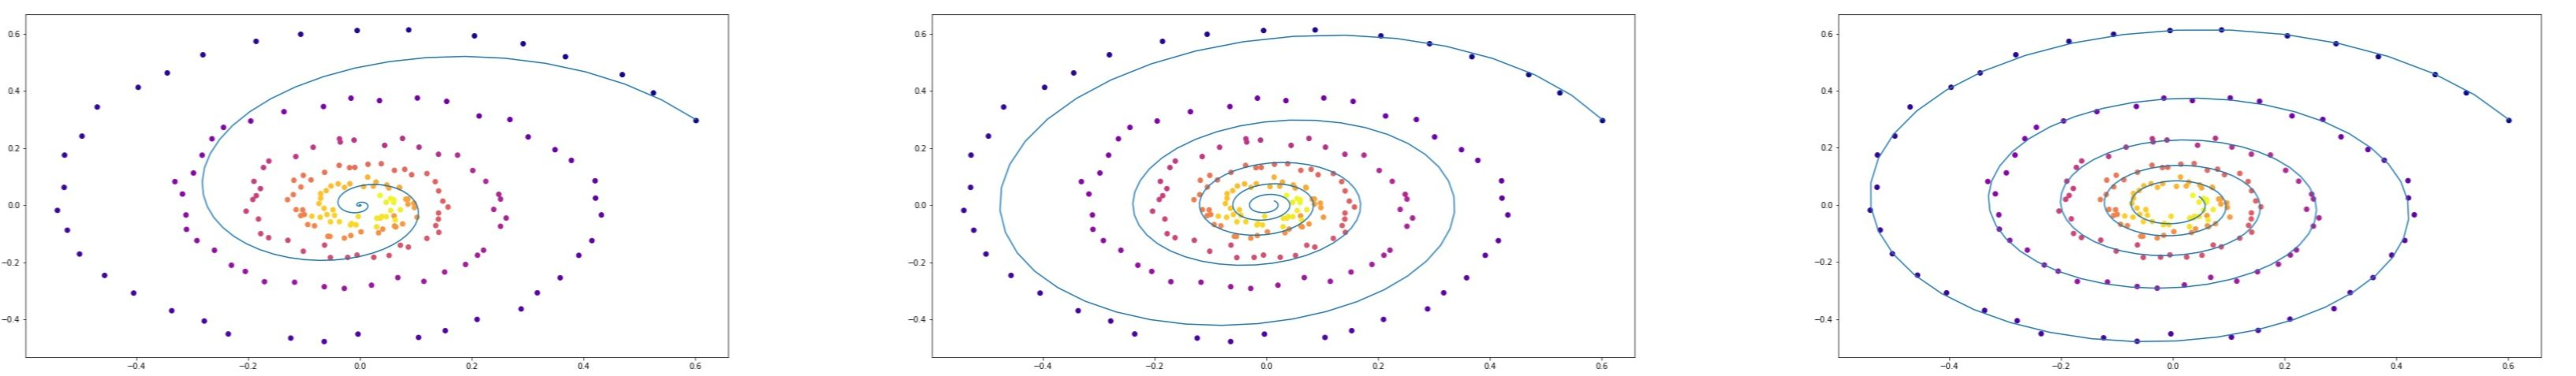
\includegraphics[width = 1\linewidth]{figures/merge_linear.jpg}
\caption{The linear function of dynamics}
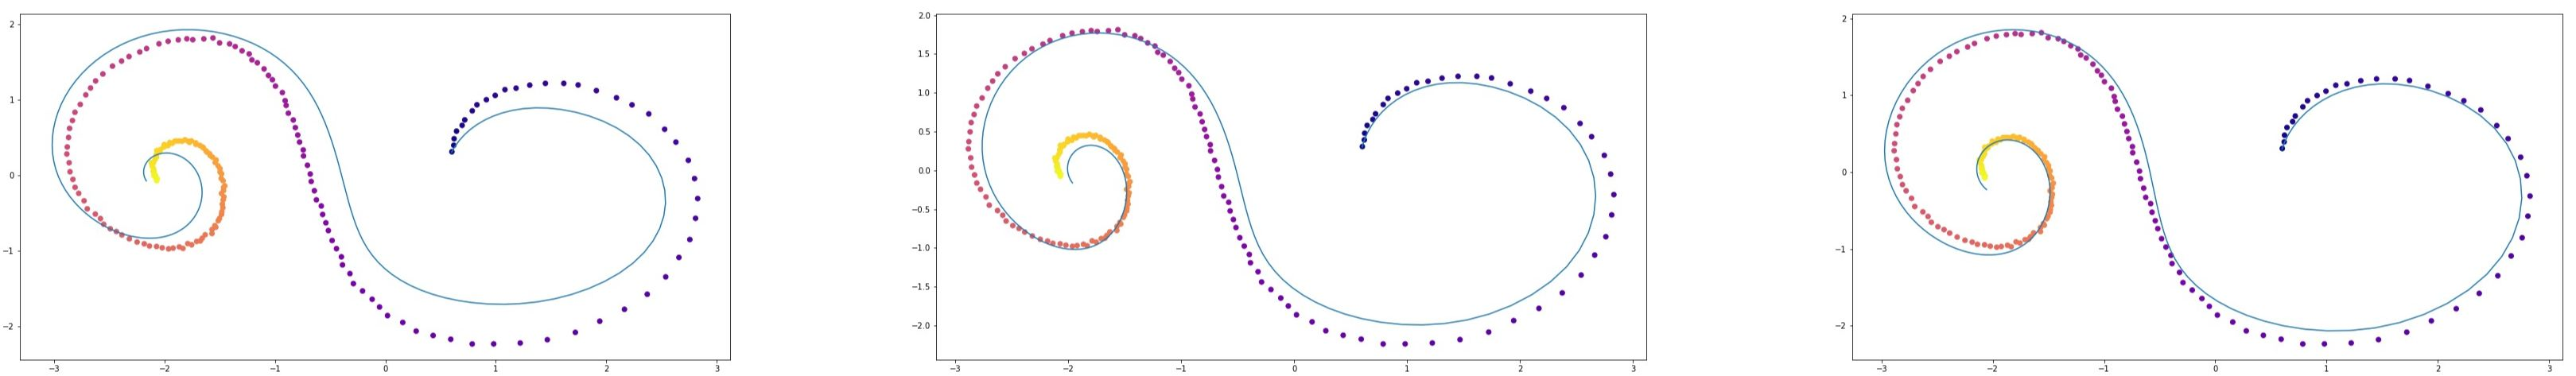
\includegraphics[width = 1\linewidth]{figures/merge_nolinear.jpeg}
\caption{The nonlinear function of dynamics}
\end{figure} 

In the first case the ODE is $z' = A z$ when $A$ is constant matrix, in the second case the ODE is $z = \sigma( <x, x_0> ) A (x-x_0) + \sigma(-<x, x_0> ) B ( x + x_0 ) $ when $\sigma$ is sigmoida, $A, B$ are constant matrix and $x_0$ is constant vector. In \cite{my_git} you can see gif images of restoring processes.
 
\medskip
\hrule\medskip
\Head{MNIST test}\\
The first experiments were devoted replay to classic MNIST test of recognizing numbers. In figure 4 we can see result of this experiment from \cite{NeuralODE}. We get the similar results.

\begin{wrapfigure}{r}{0.6\linewidth}
\centering
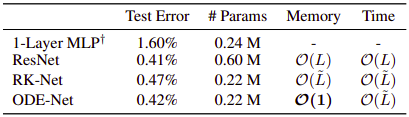
\includegraphics[width = 1\linewidth]{figures/MNIST_test.png}
\caption{}
\end{wrapfigure} $L$ denotes the number of layers in the ResNet, and $\tilde{L}$ is the number of function evaluations that the ODE solver requests in a single forward pass, which can be interpreted as an implicit number of layers.

Our experiments demonstrate that it takes 4 times longer for NeuralODE to achieve equivalent results with ResNet, but at the same time NeuralODE requires 3 times less trainable parameters and a constant quantity of memory.
\end{textblock}

\begin{textblock}{7.0}(16,1.2)
Let's note a few more of our observations. Firstly, RK-net is NeuralOde but we don't solve adjoint task (2), but use the values obtained during forward propagation. This reduces the time by about half, but increases the cost of memory up to $O(\tilde{L})$. Secondly, the time cost of training of NeuralODE directly depends on the solution of ODE (1), (2) method used and the value of its step. The experiment clearly shows the obvious linear dependence of time on the number of stages $k$ of the Runge-Kutta method and the smallness $h^{-1}$ of the step, in other words $O(k/h)$. The dependence of accuracy on the method and the step size will be examined in detail later. Negative observation, an increase in the order of the Runge-Kutta method has little effect on the accuracy of recognition of the test sample.
\hrule\medskip
\Head{Conditional normalizing flows}\\
\cite{author_git} contains some examples of working of CNF in case two-dimensional, in \cite{P_CNF} CNF method is used for sampling in three-dimensional case, see figures 5, 6. 
\begin{center}
\begin{minipage}[h]{0.49\linewidth}
\begin{figure}
\centering
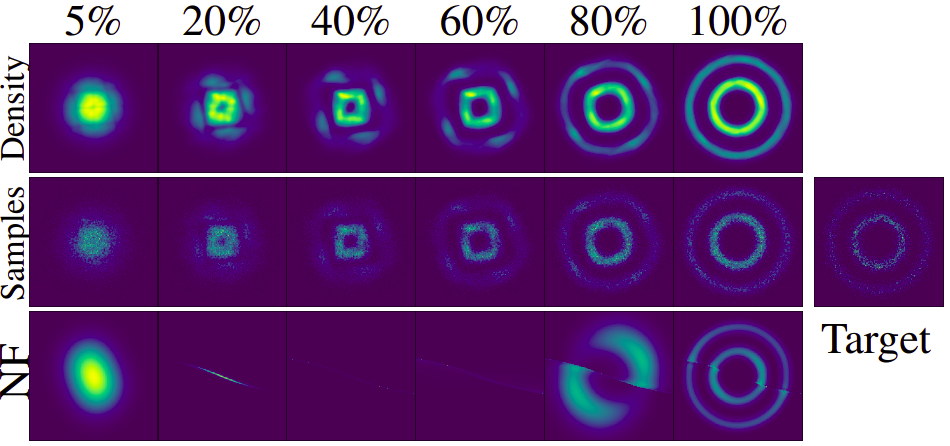
\includegraphics[width = \linewidth]{figures/CNF_NF.png}
\caption{}
\end{figure}
\end{minipage}
\hfill
\begin{minipage}[h]{0.49\linewidth}
\begin{figure}
\centering
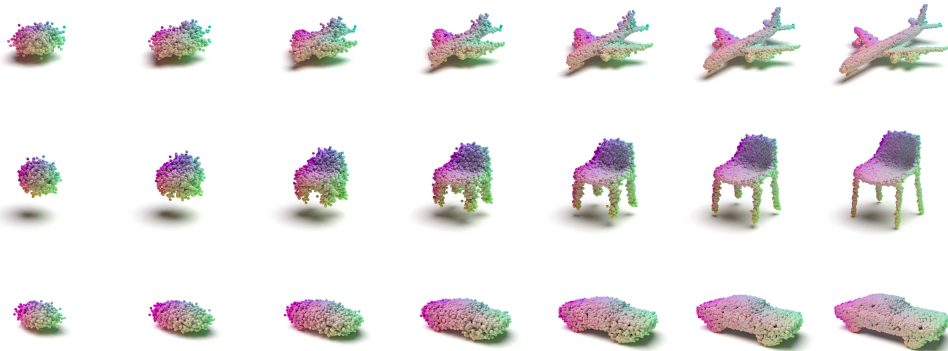
\includegraphics[width = \linewidth]{figures/CNF_stuff.png}
\caption{}
\end{figure}
\end{minipage}
\end{center}
More gifs can be found in \cite{my_git}.
\medskip
\hrule\medskip
\Head{Conclusion}\\
During our experiments, we partially tested some of the advantages and possible applications of NeuralODE. We got positive results on the MNIST test and in the task of restoring hidden dynamics in the case of a stable system, it was mentioning that NeuralODE did a good result even with non-linear dynamics. We produced the tests with CNF and get positive results in 2-dimensional and 3-dimensional cases.

\medskip
\hrule\medskip
\Head{Acknowledgements}\\
This material is based on paper \cite{NeuralODE}. The source code of the neural network was taken from \cite{author_git}. The code from \cite{habr_git} turned out very helpful because it contains all code in one python notebook. Paper \cite{P_CNF} contains code with applying CNF method in three-dimensional case. I would like to express my special gratitude to Daniil Merkulov for him initiative to make this project, references and advices.
\bibliographystyle{unsrt}
\bibliography{biblio}
\end{textblock}

\end{document}